\documentclass{beamer}
\beamertemplatenavigationsymbolsempty
\usecolortheme{beaver}
\setbeamertemplate{blocks}[rounded=true, shadow=true]
\setbeamertemplate{footline}[page number]

\usepackage[utf8]{inputenc}
\usepackage[english]{babel}
\usepackage{amssymb,amsfonts,amsmath,mathtext}
\usepackage{graphicx}
\usepackage{subfigure}
\usepackage{tikz}
\usepackage{array}
\usepackage{multicol}
\usepackage{hyperref}
\usepackage{algorithm}
\usepackage{algpseudocode}

% Your figures are here:
\graphicspath{ {fig/} {../figures/} }

%----------------------------------------------------------------------------------------------------------
\title[Deep Reference Priors]{Gibbs-Based Information Criteria and the
Over-Parameterized Regime}
\author[Y. Gao et al.]{Haobo Chen, Yuheng Bu, Gregory W.Wornell}

\date{\footnotesize

\par\bigskip\small Presented by: Papay Ivan}
%----------------------------------------------------------------------------------------------------------
\begin{document}
%----------------------------------------------------------------------------------------------------------
\begin{frame}
\thispagestyle{empty}
\maketitle
\end{frame}
%-----------------------------------------------------------------------------------------------------

\begin{frame}{Preliminaries}

Let $S=\{Z_i\}_{i=1}^n$, where $Z_i=\{(X_i,Y_i)\} \in \mathcal{Z}$ i.i.d. from the data distribution $P_Z$ with realization $z^n=(x^n,y^n)$

Parameter fo a machine learning model $w \in \mathcal{W}$

Performance of model is measured by loss function $L: \mathcal{W} \times \mathcal{Z} \rightarrow \mathbb{R}$ and the log loss $L_{log}(w,z)=-log P(y|x;w)$

Define empirical risk and the population risk:

\[
L_E(w,z^n)=\frac{1}{n} \sum_{i=1}^n L(w,z_i)
\]

\[
L_P(w,P_Z)=\mathbb{E}_{P_Z}[L(w,Z)]
\]

Here we can just take $\hat{W}_{ML} = argmax_w \hat{L}(w)=argmax_w \sum_{i=1}^n log P_k(y_i|x_i;w)$

$\overline{gen}(P_{\hat{W}|S},P_S)=\mathbb{E}_{P_{\hat{W},S}} [L_P (\hat{W}, P_Z)-L_E(\hat{W}, S)]$

Here $P_{\hat{W},S} = P_{\hat{W}|S} \otimes P_S$

\end{frame}


\begin{frame}{Classical forms of AIC and BIC}

$K$ candidate models $M_1,M_2,\dots,M_K$

Each $M_k$ defined by $P_k(y|x;\theta_k)$ and $\pi_k(\theta_k)$, where $\theta_k \in \mathcal{W}_k \in \mathbb{R}^{p_k}$


\begin{block}{AIC}
Minimize $L_P$ based on $D_{KL}$(from now just $D$) between $P_Z$ and parametric distribution

$argmin_k D(P_Z||P_k(y|x;\hat{\theta}_{ML}^{(k)}))=argmin_k \mathbb{E}_{p_Z}[-logP_k(y|x;\hat{\theta}_{ML}^{(k)})]=argmin_k L_P(\hat{\theta}_{ML}^{(k)}, P_Z)$; $AIC=-\frac{\hat{L}(\hat{\theta}_{ML})}{n} + \frac{p}{n}$

\end{block}

\begin{block}{BIC}
Minimize $L_E$ approximating the marginal likelihood of observing $z^n$ fro $M_k$ i.e. $m_k(z^n)=\int P_k(y^n|x^n;\theta_k) \pi_k(\theta_k) d \theta_k$

Laplace gives $log m_k(z^n) = \hat{L}_k(\hat{\theta}_{ML}^{(k)})-\frac{p_k}{2} log n+ O(1),n \rightarrow \infty$

$BIC=-\frac{\hat{L}(\hat{\theta}_{ML})}{n}+\frac{p log n}{2n}$

\end{block}

\end{frame}

\begin{frame}{Information Risk Minimization and Gibbs Algorithm}

\begin{block}{Lemma 1}
Suppose $L(w,z) \in [0,1]$ is bounded, and $S=\{Z_i \}_{i=1}^n$ contains $n$ i.i.d. training samples, then $|\overline{gen}(P_{\hat{W}|S}, P_S)| \le \sqrt{I(\hat{W};S) / (2n)}$
\end{block}

This brings us $P^*_{\hat{W}|S} = argmin_{P_{\hat{w}|S}} \mathbb{E}_{P_{\hat{W},S}} [L_E(\hat{W},S)] + \frac{1}{\beta} I(\hat{W};S)$ with $D(P_{\hat{W}|S} || \pi |P_S) \ge I(\hat{W};S)$

\begin{block}{Lemma 2}
    $min_{P_{\hat{w}|S}} \mathbb{E}_{P_{\hat{W},S}} [L_E(\hat{W},S)] + \frac{1}{\beta} D(P_{\hat{W}|S} || \pi |P_S)=-\frac{1}{\beta} \mathbb{E}_{P_S} [log \mathbb{E}_{\pi}[e^{-\beta L_E(W,S)}]]$

    which can be achieved by Gibbs algorithm

    $P^*_{\hat{W}|S}(w|s)=\frac{\pi(w) e^{-\beta L_E(w,s)}}{\mathbb{E}_{\pi}[e^{-\beta L_E(W,s)}]}$ for $\beta>0$
\end{block}

\end{frame}

\begin{frame}{ Sampling Algorithms for Gibbs distribution}

It is hard to compute $\mathbb{E}_{\pi}[e^{-\beta L_E(W,s)}]$ directly

\begin{block}{SGLD}
$\hat{W}_{t+1} = \hat{W}_t - \eta \nabla L_E(\hat{W}_t,s)+\sqrt{\frac{2 \eta}{\beta}} ζ_t$ where $ζ_t \sim \mathcal{N}(0, I)$

It was shown that under some conditions Wasserstein distance between induced distribution and Gibbs distribution will converge to zero as $t \rightarrow \infty$
\end{block}


\begin{block}{MALA}
Metropolis-adjusted Langevin algorithm also is first-order sampling method. Difference in additional Metropolis-adjusted step, which provides a faster convergence rate
\end{block}

\end{frame}

\begin{frame}{Experimental Results}

\begin{figure}
    \centered
    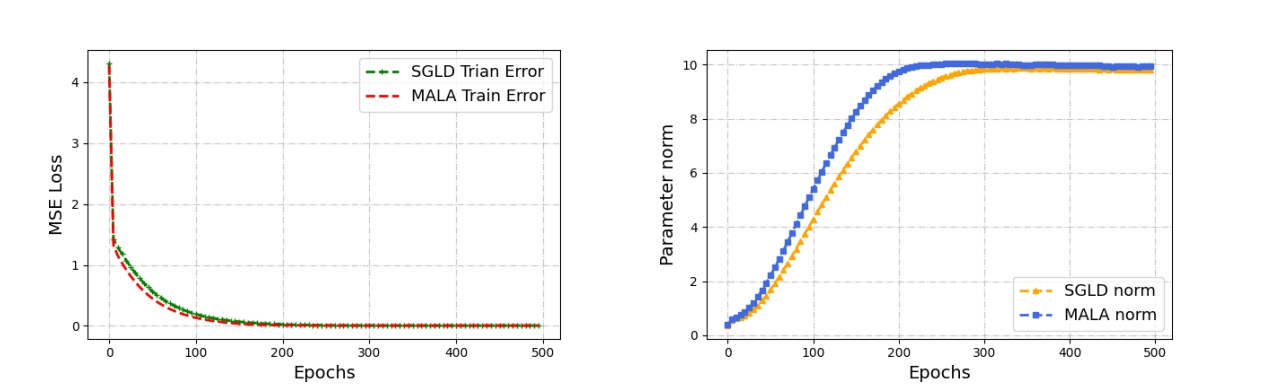
\includegraphics[width=1.0\textwidth]{sample_comparison.jpg}
    
\end{figure}

\end{frame}

\begin{frame}{Gibbs-based AIC}

\begin{block}{Proposition 1}
For the Gibbs algorithm $P^*_{\hat{W}|S}$, the expected generalization error is:
\[
\overline{gen}(P^*_{\hat{W}|S},P_S) = \frac{I_{\text{SKL}}(P^*_{\hat{W}|S}, P_S)}{\beta}
\]
\[
I_{\text{SKL}}(P_{Y|X}, P_X) \triangleq D(P_{X,Y} \| P_X \otimes P_Y) + D(P_X \otimes P_Y \| P_{X,Y})
\]
\end{block}

This leads to the \textbf{Gibbs-based AIC}:
\[
\text{AIC}^{+} \triangleq L_E(\hat{W}_{\text{Gibbs}}, \bm{z}^n) + \frac{1}{\beta} I_{\text{SKL}}(P^*_{\hat{W}|S}, P_S)
\]

\begin{block}{Theorem 1 (Classical Regime)}
$\beta = n$, $p$ is fixed and $n \to \infty$:
\[
\text{AIC}^{+} = L_E(\hat{W}_{\text{Gibbs}}, \bm{z}^n) + \frac{p}{n}
\]
\end{block}

\end{frame}

%----------------------------------------------------------------------------------------------------------
\begin{frame}{Gibbs-based BICs}

\begin{block}{Proposition 2}
For the Gibbs algorithm $P^*_{\hat{W}|S}$ with log-loss and $\beta = n$, the negative log-marginal likelihood is:
\[
-\frac{1}{n} \log m(\bm{z}^n) = \mathbb{E}_{P^*_{\hat{W}|S=\bm{z}^n}}[L_E(\hat{W}, \bm{z}^n)] + \frac{1}{n} D(P^*_{\hat{W}|S=\bm{z}^n} \| \pi)
\]
\end{block}

This motivates two versions of \textbf{Gibbs-based BIC}:
\begin{align*}
\text{BIC}^{+} &\triangleq L_E(\hat{W}_{\text{Gibbs}}, \bm{z}^n) + \frac{1}{n} D(P^*_{\hat{W}|S=\bm{z}^n} \| \pi) \\
\text{BIC}^{-} &\triangleq \mathbb{E}_{\pi}[L_E(W, \bm{z}^n)] - \frac{1}{n} D(\pi \| P^*_{\hat{W}|S=\bm{z}^n})
\end{align*}

\begin{block}{Theorem 2 (Classical Regime)}
For $p$ fixed and $n \to \infty$:
\[
\text{BIC}^{+} = L_E(\hat{W}_{\text{Gibbs}}, \bm{z}^n) + \frac{p \log n}{2n}
\]
\end{block}

\end{frame}

%----------------------------------------------------------------------------------------------------------
\begin{frame}{Over-Parameterized Regime and Random Feature Model}

\begin{block}{Key Problem}
Classical AIC/BIC fail in over-parameterized regime ($p > n$) due to:
\begin{itemize}
    \item Asymptotic normality of MLE breaks down
    \item Laplace approximation invalid
    \item Infinite number of interpolating solutions
\end{itemize}
\end{block}

\begin{block}{Random Feature (RF) Model}
Two-layer neural network with fixed first layer:
\[
g(\bm{x}) = \sum_{j=1}^{p} f\left(\frac{\langle \bm{x}, \bm{F}_j \rangle}{\sqrt{d}}\right) w_j = f\left(\frac{\bm{x}^\top \bm{F}}{\sqrt{d}}\right) \bm{w}
\]
where $\bm{F}$ is random feature matrix with i.i.d. $\mathcal{N}(0,1)$ entries.
\end{block}

Gibbs posterior for RF model is Gaussian: $P^*_{W|S} \sim \mathcal{N}(\hat{W}_\lambda, \bm{\Sigma}_w)$

\end{frame}

%----------------------------------------------------------------------------------------------------------
\begin{frame}{Over-Parameterized Gibbs-Based BICs}

For RF model, KL divergences have closed forms:

\begin{block}{BIC$^{+}$ for RF Model}
\[
\text{BIC}^{+} \triangleq L_E(\hat{W}_{\text{Gibbs}}, \bm{z}^n) + \underbrace{\frac{\lambda}{2\sigma^2} \|\hat{W}_\lambda\|_2^2}_{\ell_2 \text{ term}} + \underbrace{\frac{1}{2}V(1/\lambda, r) - \frac{\lambda}{8} \mathcal{F}(1/\lambda, r)}_{\text{covariance term}}
\]
where $r = p/n$, and $\mathcal{F}$, $V$ are defined via random matrix theory.
\end{block}



$\text{BIC}^{-} \triangleq \mathbb{E}_{\pi}[L_E(W, \bm{z}^n)] - \frac{1}{2n} \hat{W}_\lambda^\top (\bm{\Sigma}_w)^{-1} \hat{W}_\lambda - \frac{1}{2n} \operatorname{tr}(\bm{I}_p + \frac{1}{\lambda n} \bm{B}^\top \bm{B}) + \frac{1}{2} V(1/\lambda, r) + \frac{p}{2n}$


\end{frame}

%----------------------------------------------------------------------------------------------------------
\begin{frame}{Experimental Results}

\begin{figure}
    \centered
    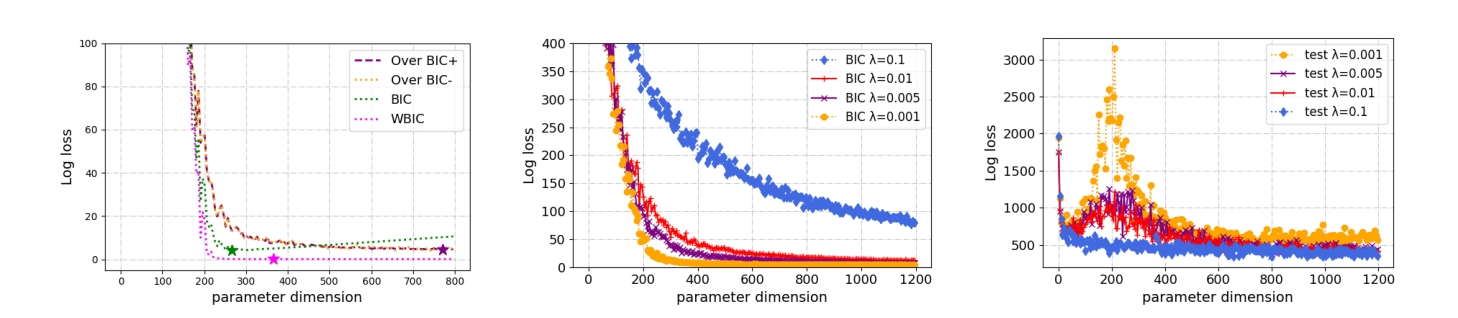
\includegraphics[width=1.0\textwidth]{BIC_comparison.jpg}
    
\end{figure}

\begin{figure}
    \centered
    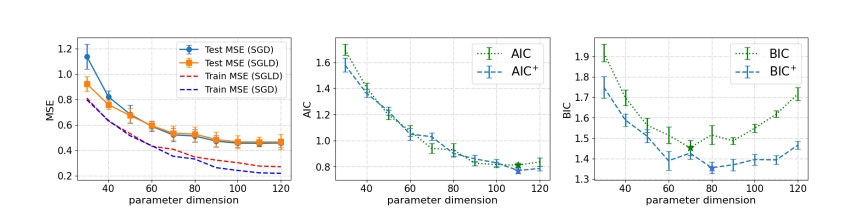
\includegraphics[width=1.0\textwidth]{double_descent.jpg}
    
\end{figure}


\end{frame}

\begin{frame}{Experimental Results}

\begin{figure}
    \centered
    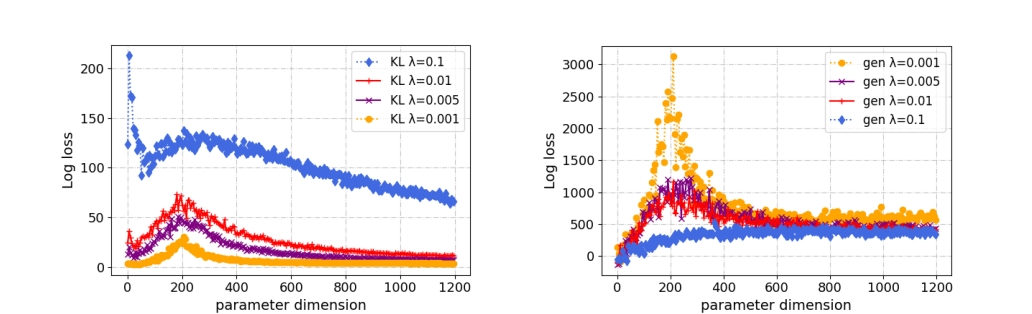
\includegraphics[width=1.0\textwidth]{kl_div.jpg}
    
\end{figure}

\begin{figure}
    \centered
    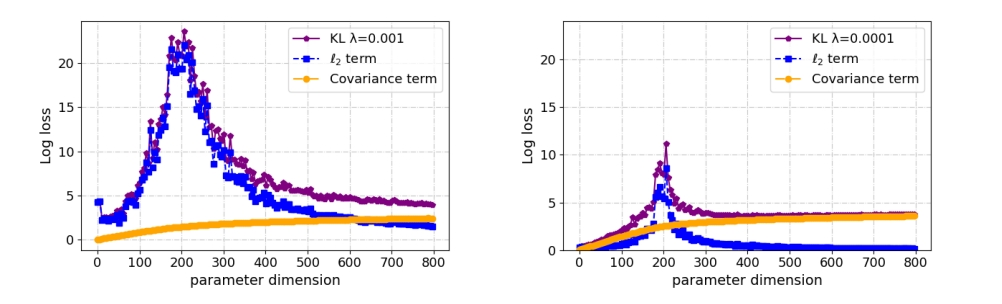
\includegraphics[width=1.0\textwidth]{cov_div.jpg}
    
\end{figure}


\end{frame}

%----------------------------------------------------------------------------------------------------------
\begin{frame}{Key Findings}

\begin{block}{Mismatch Between BIC and Population Risk}
\begin{itemize}
    \item BIC$^{+}$ does \textbf{not} exhibit double-descent behavior
    \item Marginal likelihood (BIC) and generalization error (AIC) behave differently
    \item Prior distribution ($\lambda$) significantly affects this mismatch
\end{itemize}
\end{block}

\begin{block}{Similarity Between KL Divergence and Generalization}
\begin{itemize}
    \item For fixed $\lambda$, KL divergence and $I_{\text{SKL}}$ show similar trends
    \item $\ell_2$ norm of weights decreases with over-parameterization
    \item Smaller $\ell_2$ norm correlates with better generalization
\end{itemize}
\end{block}

\end{frame}

%----------------------------------------------------------------------------------------------------------
\begin{frame}{Conclusion}

\begin{block}{Contributions}
\begin{enumerate}
    \item Developed Gibbs-based AIC/BIC using information-theoretic analysis
    \item Extended analysis to over-parameterized regime for RF models
    \item Provided exact characterization of marginal likelihood via information measures
    \item Demonstrated mismatch between marginal likelihood and generalization error
\end{enumerate}
\end{block}

\begin{block}{Implications}
\begin{itemize}
    \item Gibbs-based criteria provide unified framework for classical and over-parameterized regimes
    \item Model selection requires careful consideration of prior in over-parameterized setting
    \item Information measures offer insights into double-descent phenomena
\end{itemize}
\end{block}

\end{frame}

%----------------------------------------------------------------------------------------------------------


%----------------------------------------------------------------------------------------------------------
\end{document}